
\subsubsection{Partie commune}

Afin de faciliter l'implémentation de la version locale et distante du projet Android,
nous avons défini un socle commun aux deux versions.

Une interface \textit{ISIG1337} contenant des méthodes nécessaire à l'application telles que load,
getStructureId, getStructureName et getItineraire.
Cette interface est directement implémentée par la classe abstraite \textit{SIG1337Base},
fournissant quelques méthodes de l'interface.

\begin{figure}[H]
\centering
\resizebox{\linewidth}{!}{
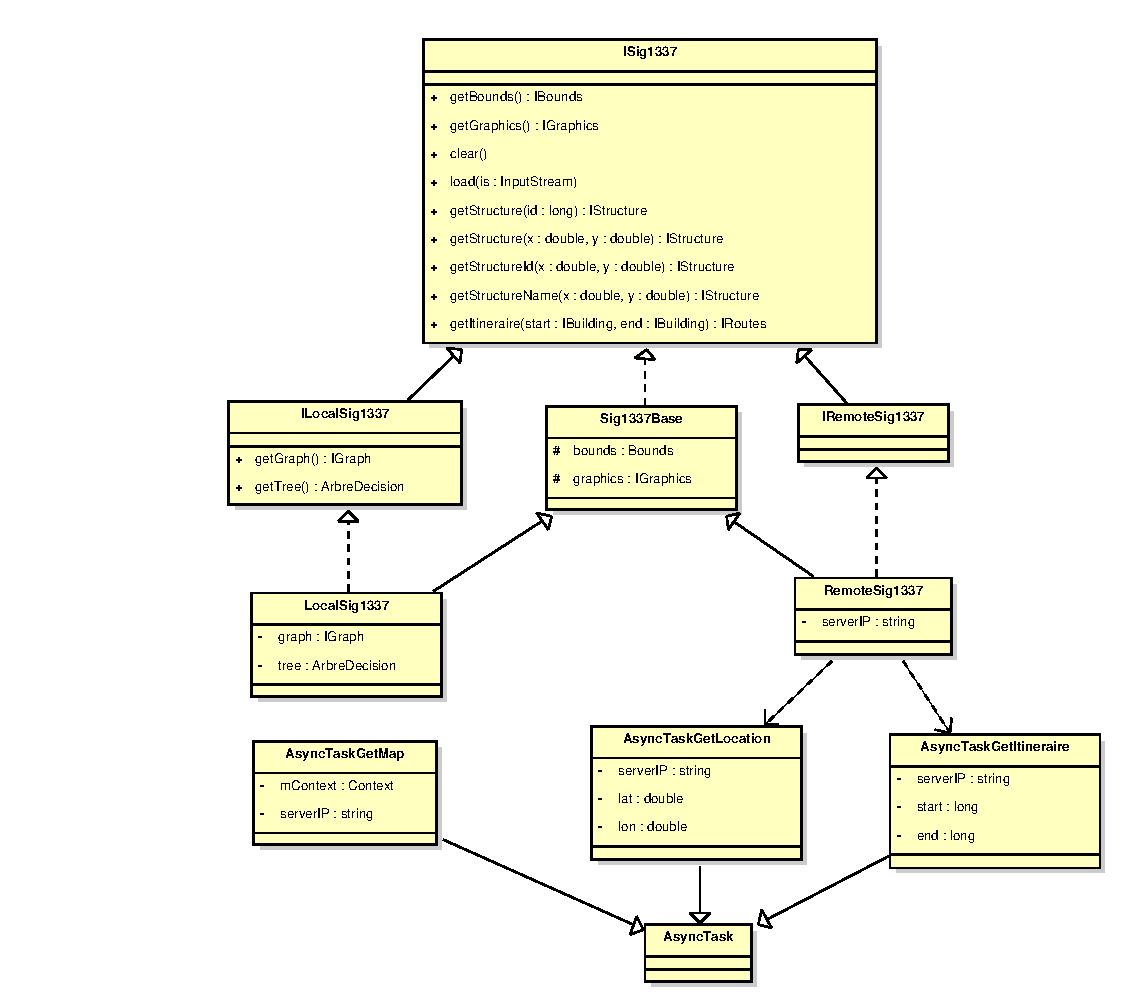
\includegraphics{../images/androidSIG.pdf}
}
\caption{Activités Android}
\end{figure}


\subsubsection{Version locale}

Pour la version locale, nous avons créé \textit{LocalActivity} qui hérite de \textit{ActivityBase}.
Elle contient une instance de \textit{LocalSIG1337}, qui hérite de \textit{SIG1337Base} et qui implémente \textit{ILocalSIG1337}.
Cette dernière possède les méthodes getGraph et getTree, permettant respectivement de récupérer le graphe et l'arbre de décision.

La méthode loadSIG1337() qui doit charger le SIG va charger le xml qui avait été généré précédemment dans le projet \textit{Commun}
et qui a été placée dans les fichiers de l'application.
Ce fichier, en version locale, contient la carte au format xml, le graphe et l'arbre de décision.

Lorsqu'on touche un bâtiment sur la carte, un calcul est fait sur l'arbre de décision qui renvoie finalement le nom du dit bâtiment.

Pour le calcul d'itinéraire, une fois les deux bâtiments sélectionnés via \textit{ItineraireActivity} et le bouton validé,
l'application fait appel au graphe afin de calculer l'itinéraire entre ces deux bâtiments.


\subsubsection{Version distante}

Pour la version distante, nous avons créé \textit{RemoteActivity} qui hérite de \textit{ActivityBase}.
Elle contient une instance de \textit{RemoteSIG1337}, qui hérite de \textit{SIG1337Base} et possède un attribut serverIP,
permettant d'avoir l'adresse du serveur.

La méthode loadSIG1337() qui doit charger le SIG fait appel à une instance de la classe \textit{AsyncTastGetMap},
qui hérite de \textit{AsyncTask}.
Cette tâche asynchrone fait appel, via une requête http, au WebService hébergé sur un serveur distant.
Le serveur renvoie la carte au format xml allégé de l'arbre de décision.
Une fois la réponse du serveur récupérée, la méthode createMap de l'activité est appelée et charge la carte en mémoire.

Lorsqu'on touche la carte un court instant, une requête est envoyée au WebService,
via une instance de la classe \textit{AsyncTaskGetLocation},
qui va récupérer les informations de base du bâtiment le plus proche de l'endroit que l'on a touché, au format JSON.
La tâche asynchrone va récupérer ce JSON, le parser et afficher un Toast avec le nom du bâtiment.

Pour le calcul d'itinéraire, une fois les deux bâtiments sélectionnés via \textit{ItineraireActivity} et le bouton validé,
l'application fait appel à une instance de \textit{AsyncTaskGetItineraire},
qui va demander au WebService de calculer le chemin le plus court entre les deux bâtiments.
La réponse est renvoyée au format JSON afin de pouvoir être parsée facilement via l'application.
Celle-ci va ensuite ajouter un chemin du bâtiment de départ au bâtiment d'arrivée sur la carte.


